\documentclass[notheorems]{beamer}
% \documentclass{beamer}

\mode<presentation>
{
  % \usetheme{default}
  \usetheme{Antibes}
  \setbeamertemplate{footline}[frame number]{}
  \setbeamertemplate{navigation symbols}{}
}

\usepackage{amsmath}
\usepackage{ragged2e}
\justifying\let\raggedright\justifying

\makeatletter
\newenvironment<>{proofs}[1][\proofname]{
    \par
    \def\insertproofname{#1\@addpunct{.}}
    \usebeamertemplate{proof begin}#2}
  {\usebeamertemplate{proof end}}

  \newenvironment<>{solution}[1][Solution.]{
    \par
    \def\insertproofname{#1\@addpunct{.}}
    \usebeamertemplate{proof begin}#2}
  {\usebeamertemplate{proof end}}

  \newtheorem*{definition}{Definition}
  \newtheorem{example}{Example}[section]
  \newtheorem{theorem}{Theorem}[section]
  \newtheorem{property}{Property}[section]
\makeatother

\setbeamertemplate{theorems}[numbered]
% \setbeamertemplate{definition}[nonumbered]

\setbeamertemplate{section in toc}[sections numbered]
\setbeamertemplate{subsection in toc}[subsections numbered]
% \setbeamertemplate{subsubsection in toc}[subsubsections numbered]

\numberwithin{equation}{section}
\numberwithin{equation}{subsection}

\usefonttheme[onlymath]{serif}
\providecommand{\Arg}{\operatorname{Arg}}
\providecommand{\Ln}{\operatorname{Ln}}
\providecommand{\Arcsin}{\operatorname{Arcsin}}
\providecommand{\Arccos}{\operatorname{Arccos}}
\providecommand{\Arctan}{\operatorname{Arctan}}
\providecommand{\Arcsinh}{\operatorname{Arcsinh}}
\providecommand{\Arccosh}{\operatorname{Arccosh}}
\providecommand{\Arctanh}{\operatorname{Arctanh}}

% \providecommand{\abs}[1]{\lvert#1\rvert}
\providecommand{\abs}[1]{\left\lvert#1\right\rvert}
% \providecommand{\norm}[1]{\lVert#1\rVert}

\title{Chapter 2: Complex Functions}
\author{Taotao Wang, Associate Professor}
\institute{College of Electronics and Information Engineering, Shenzhen University}
% \date{\today}

\begin{document}

\everymath{\displaystyle}

\begin{frame}
	\titlepage
\end{frame}

\begin{frame}{Outline}
	\tableofcontents
\end{frame}

\section{Concept of Analytic Functions}

\begin{frame}
	\frametitle{Outline}
	\tableofcontents[currentsection]
\end{frame}

\begin{frame}
	\begin{enumerate}
		\item \textbf{Derivatives of Complex Functions}
		      \begin{enumerate}[1)]
			      \item Definition of Derivative
			            \begin{definition}
				            Suppose that the function $w=f(z)$ is defined in the domain $D$, the point $z_0$ is in $D$, and $z_0+\Delta z$ is also in $D$. When $z_0+\Delta z\to z_0$ (that is, $\Delta z\to 0$), if the limit
				            \[\lim_{\Delta z\to 0}\frac{f(z_0+\Delta z)-f(z_0)}{\Delta z}\]
				             exists, then $f(z)$ is said to be differentiable at $z_0$.
			            \end{definition}
		      \end{enumerate}
	\end{enumerate}
\end{frame}

\begin{frame}
	\begin{enumerate}
		\setcounter{enumi}{1}
		\item []
		      \begin{enumerate}[1)]
			      \item []
			            \begin{definition}
				            This limit value is called the derivative of $f(z)$ at $z_0$, denoted as
				            \[f'(z_0)=\left.\frac{\mathrm{d}w}{\mathrm{d}z}\right|_{z=z_0}=\lim_{\Delta z\to 0}\frac{f(z_0+\Delta z)-f(z_0)}{\Delta z}. \tag{2.1.1}\]
				            The definition means that for any given $\varepsilon>0$, there is a corresponding $\delta(\varepsilon)>0$, so that when $0<|\Delta z|<\delta$, we have
				            \[\abs{\frac{f(z_0+\Delta z)-f(z_0)}{\Delta z}-f'(z_0)}<\varepsilon.\]
			            \end{definition}
		      \end{enumerate}
	\end{enumerate}
\end{frame}

\begin{frame}
	\begin{example}
		Determine whether the following functions are differentiable.
		\begin{enumerate}
			\item $f(z)=z^2$;
			\item $f(z)=2x+yi$.
		\end{enumerate}
	\end{example}
	\begin{solution}<2->
		\begin{enumerate}
			\item For any point $z$ in the complex plane, the limit
			      \begin{align*}
				      \lim_{\Delta z\to 0}\frac{f(z+\Delta z)-f(z)}{\Delta z} & =\lim_{\Delta z\to 0}\frac{(z+\Delta z)^2-z^2}{\Delta z} \\
				                                                              & =\lim_{\Delta z\to 0}(2z+\Delta z)                       \\
				                                                              & =2z
			      \end{align*}
		\end{enumerate}
	\end{solution}
\end{frame}

\begin{frame}
	\begin{solution}[Solution\ (Cont.)]
		\begin{enumerate}
			\setcounter{enumi}{1}
			\item []
			      So $f(z)=z^2$ is differentiable everywhere in the complex plane, and its derivative is $f'(z)=2z$
			\item \resizebox*{\linewidth}{!}{
				      \begin{minipage}{\linewidth}
					      \begin{align*}
						      \lim_{\Delta z\to 0}\frac{f(z+\Delta z)-f(z)}{\Delta z} & =\lim_{\Delta z\to 0}\frac{2(x+\Delta x)+(y+\Delta y)i-(2x+yi)}{\Delta x+\Delta yi} \\
						                                                              & =\lim_{\Delta z\to 0}\frac{2\Delta x+\Delta yi}{\Delta x+\Delta yi}
					      \end{align*}
				      \end{minipage}
			      }
		\end{enumerate}
	\end{solution}
\end{frame}

\begin{frame}
	\begin{solution}[Solution\ (Cont.)]
		\begin{enumerate}
			\setcounter{enumi}{2}
			\item []
			      For any point $z$ in the complex plane, when $z+\Delta z$ approaches $z$ along a straight line parallel to the $x$-axis (see Figure 2.1), we have $\Delta y=0$ and the limit is given by
			      \[\lim_{\Delta z\to 0}\frac{2\Delta x+\Delta yi}{\Delta x+\Delta yi}=\lim_{\Delta z\to 0}\frac{2\Delta x}{\Delta x}=2.\]
			      However, when $z+\Delta z$ approaches $z$ along a straight line parallel to the $y$ axis, we have $\Delta x=0$, and the limit is given by
			      \[\lim_{\Delta z\to 0}\frac{2\Delta x+\Delta yi}{\Delta x+\Delta yi}=\lim_{\Delta z\to 0}\frac{\Delta yi}{\Delta yi}=1.\]
			      The above is to say when $z+\Delta z$ approaches $z$ in different directions, the limit is different. Thus, the derivative of $f(z)=2x+yi$ does not exist.
		\end{enumerate}
	\end{solution}
\end{frame}

\begin{frame}
	\begin{solution}[Solution\ (Cont.)]
		\begin{enumerate}
			\setcounter{enumi}{2}
			\item []
			      \begin{figure}
				      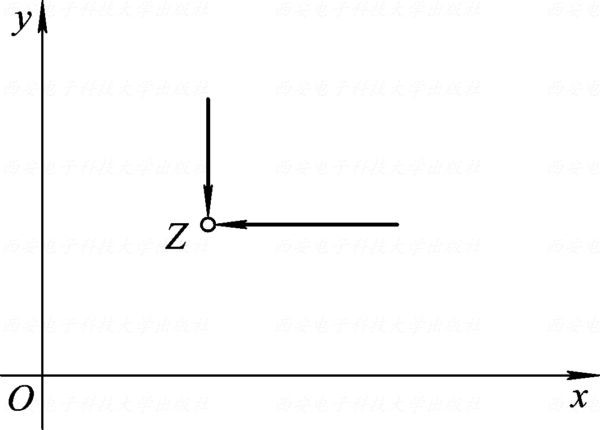
\includegraphics[height=0.6\textheight]{Figure_2_1.jpg}
				      \caption{2.1}
			      \end{figure}
		\end{enumerate}
	\end{solution}
\end{frame}

\begin{frame}
	\begin{enumerate}
		\setcounter{enumi}{1}
		\item []
		      \begin{enumerate}[1)]
			      \setcounter{enumii}{1}
			      \item Differentiability and Continuity\\
			            First, we consider the case where $f(z)$ is differentiable at a point $z_0$. According to the definition of derivative, for any given $\varepsilon>0$, there is a $\delta(\varepsilon)>0$, so that when $0<|\Delta z|<\delta$, we have
			            \[\abs{\frac{f(z_0+\Delta z)-f(z_0)}{\Delta z}-f'(z_0)}<\varepsilon\]
			            Let
			            \[\rho(\Delta z)=\frac{f(z_0+\Delta z)-f(z_0)}{\Delta z}-f'(z_0), \tag{2.1.2}\]
		      \end{enumerate}
	\end{enumerate}
\end{frame}

\begin{frame}
	\begin{enumerate}
		\setcounter{enumi}{1}
		\item []
		      \begin{enumerate}[1)]
			      \setcounter{enumii}{1}
			      \item []
			            then
			            \[\lim_{\Delta z\to 0}\rho(\Delta z)=0.\]
			            From equation (2.1.2), we have
			            \[f(z_0+\Delta z)=f(z_0)+f'(z_0)\Delta z+\rho(\Delta z)\Delta z, \tag{2.1.3}\]
			            which means
			            \[\lim_{\Delta z\to 0}f(z_0+\Delta z)=f(z_0),\]
			            Thus, $f(z)$ is continuous at $z_0$.
		      \end{enumerate}
	\end{enumerate}
\end{frame}

\begin{frame}
	\begin{enumerate}
		\setcounter{enumi}{1}
		\item []
		      \begin{enumerate}[1)]
			      \setcounter{enumii}{2}
			      \item Derivative Rules\\
			            Complex functions have the same derivative rules as real functions, which are given as follows:
			            \begin{enumerate}[a)]
				            \item $(c)'=0$, where $c$ is a complex constant;
				            \item $(z^n)'=nz^{n-1}$, where $n$ is a positive integer;
				            \item $[f(z)\pm g(z)]'=f'(z)\pm g'(z)$;
				            \item $[f(z)g(z)]'=f'(z)g(z)+f(z)g'(z)$;
				            \item $\left[\frac{f(z)}{g(z)}\right]'=\frac{1}{g^2(z)}[g(z)f'(z)-f(z)g'(z)], g(z)\neq 0$;
				            \item $f'[g(z)]=f'(w)g'(z)$, where $w=g(z)$;
				            \item $f'(z)=\frac{1}{\varphi'(w)}$, where $w=f(z)$ and $z=\varphi(w)$ are two single-valued functions that are inverse to each other, and $\varphi'(w)\neq 0$.
			            \end{enumerate}
		      \end{enumerate}
	\end{enumerate}
\end{frame}



\begin{frame}
	\begin{enumerate}
		\setcounter{enumi}{1}
		\item []
		      \begin{enumerate}[1)]
			      \setcounter{enumii}{3}
			      \item Definition of Differential\\
			            Like the derivative, the differential of a complex function is exactly the same in form as the differential of a real function.
			            Assuming that the function $w=f(z)$ is differentiable at $z_0$, then from equation (2.1.3) we know
			            \[\Delta w=f(z_0+\Delta z)-f(z_0)=f'(z_0)\Delta z+\rho(\Delta z)\Delta z,\]
			            where
			            \[\lim_{\Delta z\to 0}\rho(\Delta z)=0.\]
		      \end{enumerate}
	\end{enumerate}
\end{frame}

\begin{frame}
	\begin{enumerate}
		\setcounter{enumi}{1}
		\item []
		      \begin{enumerate}[1)]
			      \setcounter{enumii}{3}
			      \item []
			            Therefore, $|\rho(\Delta z)\Delta z|$ is the high-order infinitesimal of $|\Delta z|$, and $f'(z_0)\Delta z$ is the linear part of the change $\Delta w$ of the function $w=f(z)$. We call $f'(z_0)\Delta z$  the differential of the function $w=f(z)$ at the point $z_0$, denoted as
			            \[\mathrm{d}w=f'(z_0)\Delta z. \tag{2.1.4}\]
			            If the differential of the function at $z_0$ exists, then the function $f(z)$ is said to be differentiable at $z_0$. Since for $f(z)=z$, we have $\mathrm{d}z=\Delta z$, the formula (2.1.4) is written as
			            \[\mathrm{d}w=f'(z_0)\mathrm{d}z.\]
		      \end{enumerate}
	\end{enumerate}
\end{frame}

\begin{frame}
	\begin{enumerate}
		\setcounter{enumi}{1}
		\item []
		      \begin{enumerate}[1)]
			      \setcounter{enumii}{3}
			      \item []
			            That is,
			            \[f'(z_0)=\left.\frac{\mathrm{d}w}{\mathrm{d}z}\right|_{z=z_0}. \tag{2.1.5}\]
			            It can be seen the fact that the function $w=f(z)$ is differentiable at $z_0$ means the function $w=f(z)$ has  differential and derivative at $z_0$. If $f(z)$ is differentiable everywhere in domain $D$, then $f(z)$ is said to be differentiable in $D$.
		      \end{enumerate}
	\end{enumerate}
\end{frame}

\begin{frame}
	\begin{enumerate}
		\setcounter{enumi}{1}
		\item \textbf{Analytic function}
		      \begin{definition}
			      If the function $f(z)$ is differentiable everywhere in the neighborhood of $z_0$ and the point $z_0$, then $f(z)$ is said to be analytic at $z_0$. If $f(z)$ is analytic at every point in domain $D$, then $f(z)$ is said to be analytic in $D$, or $f(z)$ is an analytic function in $D$.\\
			      If $f(z)$ is not analytic at $z_0$, then $z_0$ is called the singularity of $f(z)$.
		      \end{definition}
	\end{enumerate}
\end{frame}

\begin{frame}
	\begin{example}
		Investigate the analyticity of the following functions.
		\begin{enumerate}
			\item $f(z)=z^2$;
			\item $f(z)=2x+yi$;
			\item $f(z)=\abs{z}^2$;
			\item $f(z)=1/z$.
		\end{enumerate}
	\end{example}
	\begin{solution}<2->
		From the definition of analytic function and [Example 1.1] in this chapter, we can see that $f(z)=z^2$ is analytic in the complex plane, but $f(z)=2x+yi$ is not analytic everywhere.
	\end{solution}
\end{frame}

\begin{frame}
	\begin{solution}[Solution\ (Cont.)]
		For the function $f(z)=\abs{z}^2$,
		\begin{align*}
			\frac{f(z_0+\Delta z)-f(z_0)}{\Delta z} & =\frac{\abs{z_0+\Delta z}^2-\abs{z_0}^2}{\Delta z}                                     \\
			                                         & =\frac{(z_0+\Delta z)(\overline{z_0}+\overline{\Delta z}-z_0\overline{z_0})}{\Delta z} \\
			                                         & =\overline{z_0}+\overline{\Delta z}+z_0\frac{\overline{\Delta z}}{\Delta z}
		\end{align*}
	\end{solution}
\end{frame}

\begin{frame}
	\begin{solution}[Solution\ (Cont.)]
		It is easy to know that if $z_0=0$, when $\Delta z\to 0$, the limit of the above formula is zero; if $z_0\neq 0$, let $z_0+\Delta z$ approach $z_0$ along the straight line $y-y_0=k(x-x_0)$, and
		\[\frac{\overline{\Delta z}}{\Delta z}=\frac{\Delta x-\Delta y i}{\Delta x+\Delta y i}=\frac{1-\frac{\Delta y}{\Delta x} i}{1+\frac{\Delta y}{\Delta x} i}=\frac{1-k i}{1+k i}.\]
		Due to the arbitrary $k$, the above formula does not converge to a fixed value.
	\end{solution}
\end{frame}

\begin{frame}
	\begin{theorem}
		\begin{enumerate}
			\item The sum, difference, product, and quotient (excluding the point where the denominator is zero) of the two analytic functions $f(z)$ and $g(z)$ in domain $D$ are analytic in $D$.
			\item Suppose that the function $h=g(z)$ is analytic in the domain $D$ in the $z$-plane, and the function $w=f(h)$ is analytic in the domain $G$ in the $h$-plane. If for any $z\in D$, there is $h=g(z)\in G$, then the complex function $w=f[g(z)]$ is analytic in $D$.
		\end{enumerate}
	\end{theorem}
\end{frame}


\section{Necessary and Sufficient Conditions for Analytic Functions}

\begin{frame}
	\frametitle{Outline}
	\tableofcontents[currentsection]
\end{frame}

\begin{frame}
	\begin{enumerate}
		\item \textbf{Main Theorem}
		      \begin{theorem}
			      Assuming that the function $f(z)=u(x, y)+i v(x, y)$ is defined in the domain $D$, then the necessary and sufficient condition for $f(z)$ to be differentiable at a point in $D$ is: $u(x, y)$ and $v(x, y)$ are differentiable at point $(x, y)$, and the Cauchy-Riemann equations
			      \[\frac{\partial u}{\partial x}=\frac{\partial v}{\partial y}, \quad \frac{\partial u}{\partial y}=-\frac{\partial v}{\partial x}\]
			      is satisfied at this point.
		      \end{theorem}
	\end{enumerate}
\end{frame}

\begin{frame}
	\begin{proofs}
		\begin{enumerate}
			\item Necessity.\\
			      Suppose $f(z)=u(x, y)+iv(x, y)$ is defined in the domain $D$,\\
			      and $f(z)$ is differentiable at a point $z=x+yi$ in $D$,\\
			      then for a sufficiently small $\abs{\Delta z}=\abs{\Delta x+i\Delta y}>0$,\\
			      there is $f(z+\Delta z)-f(z)=f'(z)\Delta z+\rho(\Delta z)\Delta z$,\\
			      where $\lim_{\Delta z\to 0}\rho(\Delta z)=0$.\\
			      Let $f(z+\Delta z)-f(z)=\Delta u+i\Delta v$,\\
			      $f'(z)=a+ib$, $\rho(\Delta z)=\rho_1+i\rho_2$,
		\end{enumerate}
	\end{proofs}
\end{frame}

\begin{frame}
	\begin{proofs}[Proof.\ (Cont.)]
		\begin{enumerate}
			\item []
			      So, $\begin{aligned}[t]
					      \Delta u+i\Delta v & =(a+ib)(\Delta x+i\Delta y)+(\rho_1+i\rho_2)(\Delta x+i\Delta y) \\
					                         & =(a\Delta x-b\Delta y+\rho_1\Delta x-\rho_2\Delta y)             \\
					                         & \quad+i(b\Delta x-a\Delta y+\rho_2\Delta x-\rho_1\Delta y)
				      \end{aligned}$\\
			      So, $\begin{aligned}[t]
					      \Delta u & =a\Delta x-b\Delta y+\rho_1\Delta x-\rho_2\Delta y \\
					      \Delta v & =b\Delta x+a\Delta y+\rho_2\Delta x-\rho_1\Delta y
				      \end{aligned}$\\
			      Because $\lim_{\Delta z\to 0}\rho(\Delta z)=0$, $\lim_{\substack{\Delta x\to 0\\ \Delta y\to 0}}\rho_1=\lim_{\substack{\Delta x\to 0\\ \Delta y\to 0}}\rho_2=0$,
		\end{enumerate}
	\end{proofs}
\end{frame}

\begin{frame}
	\begin{proofs}[Proof.\ (Cont.)]
		\begin{enumerate}
			\setcounter{enumi}{1}
			\item []
			      it can be seen that $u(x, y)$ and $v(x, y)$ are differentiable at point $(x, y)$ and satisfy the equations
			      \[\frac{\partial u}{\partial x}=\frac{\partial v}{\partial y}, \quad \frac{\partial u}{\partial y}=-\frac{\partial v}{\partial x}.\]
			\item Sufficiency.\\
			      Since,
			      \begin{align*}
				      f(z+\Delta z)-f(z)= & u(x+\Delta x, y+\Delta y)-u(x, y)     \\
				                          & +i[v(x+\Delta x, y+\Delta y)-v(x, y)] \\
				      =                   & \Delta u+i \Delta v
			      \end{align*}
			      and $u(x, y)$ and $v(x, y)$ are differentiable at point $(x, y)$,
		\end{enumerate}
	\end{proofs}
\end{frame}

\begin{frame}
	\begin{proofs}[Proof.\ (Cont.)]
		\begin{enumerate}
			\setcounter{enumi}{1}
			\item []
			      So, $\begin{aligned}[t]
					      \Delta u & =\frac{\partial u}{\partial x}\Delta x+\frac{\partial u}{\partial y}\Delta y+\varepsilon_1\Delta x+\varepsilon_2\Delta y \\
					      \Delta v & =\frac{\partial v}{\partial x}\Delta x+\frac{\partial v}{\partial y}\Delta y+\varepsilon_3\Delta x+\varepsilon_4\Delta y
				      \end{aligned}$\\
			      where $\lim_{\substack{\Delta x\to 0\\ \Delta y\to 0}} \varepsilon_k=0, \quad(k=1,2,3,4)$\\
			      So, $\begin{aligned}[t]
					        & f(z+\Delta z)-f(z)                                                                                                                                                  \\
					      = & \left(\frac{\partial u}{\partial x}+i\frac{\partial v}{\partial x}\right)\Delta x+\left(\frac{\partial u}{\partial y}+i\frac{\partial v}{\partial y}\right)\Delta y \\
					        & +(\varepsilon_1+i\varepsilon_3)\Delta x+(\varepsilon_2+i\varepsilon_4)\Delta y.
				      \end{aligned}$
		\end{enumerate}
	\end{proofs}
\end{frame}

\begin{frame}
	\begin{proofs}[Proof.\ (Cont.)]
		\begin{enumerate}
			\setcounter{enumi}{1}
			\item []
			      From the Cauchy-Riemann equations
			      \[\frac{\partial u}{\partial x}=\frac{\partial v}{\partial y},\quad\frac{\partial u}{\partial y}=-\frac{\partial v}{\partial x}=i^2\frac{\partial v}{\partial x}\]
			      \begin{multline*}
				      f(z+\Delta z)-f(z)=\\
				      \left(\frac{\partial u}{\partial x}+i\frac{\partial v}{\partial x}\right)(\Delta x+i \Delta y)+(\varepsilon_1+i \varepsilon_3)\Delta x+(\varepsilon_2+i \varepsilon_4)\Delta y
			      \end{multline*}
			      \begin{multline*}
				      \frac{f(z+\Delta z)-f(z)}{\Delta z}=\\
				      \frac{\partial u}{\partial x}+i\frac{\partial v}{\partial x}+(\varepsilon_1+i\varepsilon_3)\frac{\Delta x}{\Delta z}+(\varepsilon_2+i\varepsilon_4)\frac{\Delta y}{\Delta z}
			      \end{multline*}
		\end{enumerate}
	\end{proofs}
\end{frame}

\begin{frame}
	\begin{proof}[\proofname\ (Cont.)]
		\begin{enumerate}
			\setcounter{enumi}{1}
			\item []
			      Because $\abs{\frac{\Delta x}{\Delta z}}\leq 1,\abs{\frac{\Delta y}{\Delta z}}\leq 1$,\\
			      $\lim_{\Delta z\to 0}\left[(\varepsilon_1+i\varepsilon_3)\frac{\Delta x}{\Delta z}+(\varepsilon_2+i\varepsilon_4)\frac{\Delta y}{\Delta z}\right]=0$.\\
			      So, $f'(z)=\lim_{\Delta z\to 0}\frac{f(z+\Delta z)-f(z)}{\Delta z}=\frac{\partial u}{\partial x}+i\frac{\partial v}{\partial x}$.\\
			      That is, the function $f(z)=u(x,y)+iv(x,y)$ is differentiable at point $z=x+yi$.
		\end{enumerate}
	\end{proof}
\end{frame}

\begin{frame}
	\begin{enumerate}
		\item []
		 According to the proof of Theorem 2.1, the derivative of function $f(z)=u(x,y)+iv(x,y)$ at point $z=x+yi$ is
		      \[f'(z)=\frac{\partial u}{\partial x}+i\frac{\partial v}{\partial x}=\frac{1}{i}\frac{\partial u}{\partial y}+\frac{\partial v}{\partial y}\]
		      \begin{theorem}
			      The necessary and sufficient conditions for the analyticity of function $f(z)=u(x,y)+iv(x,y)$ in its defined domain $D$ are that $u(x,y)$ and $v(x,y)$ are differentiable in $D$ and satisfy Cauchy-Riemann equations.
		      \end{theorem}
	\end{enumerate}
\end{frame}

\begin{frame}
	\begin{enumerate}
		\item []
		      How to determine an analytic function:
		      \begin{enumerate}[1)]
			      \item If the derivative definition and the derivation rules can be used to prove that the derivative of the complex function $f(z)$ exists everywhere in the domain $D$, then it can be concluded that $f(z)$ is analytic in $D$.
			      \item If the first-order partial derivatives of $u$ and $v$ in $D$ in the complex function $f(z)=u+iv$ all exist, are continuous (thus $u$ and $v(x,y)$ are differentiable) and satisfy the Cauchy-Riemann equations, then according to the necessary and sufficient condition of the analytic function, we can conclude that $f(z)$ is analytic in $D$.
		      \end{enumerate}
	\end{enumerate}
\end{frame}

\begin{frame}
	\begin{enumerate}
		\setcounter{enumi}{1}
		\item \textbf{Examples}
	\end{enumerate}
	\begin{example}
		Determine where the following functions are differentiable and analytic:
		\begin{enumerate}
			\item $w=\overline{z}$;
			\item $f(z)=e^x(\cos y+i\sin y)$;
			\item $w=z\operatorname{Re}(z)$.
		\end{enumerate}
	\end{example}
	\begin{solution}<2->
		\begin{enumerate}
			\item $w=\overline{z},\quad u=x,\quad v=-y,$\\
			      $\frac{\partial u}{\partial x}=1,\quad\frac{\partial u}{\partial y}=0,\quad\frac{\partial v}{\partial x}=0,\quad\frac{\partial v}{\partial y}=-1.$\\
			      The Cauchy-Riemann equations are not satisfied, so $w=\overline{z}$ is not differentiable and analytic everywhere in the complex plane.
		\end{enumerate}
	\end{solution}
\end{frame}

\begin{frame}
	\begin{solution}[Solution\ (Cont.)]
		\begin{enumerate}
			\setcounter{enumi}{1}
			\item \[\boxed{f(z)=e^x(\cos y+i\sin y)} \tag{Exponential function}\]
			      \[u=e^x\cos y,\quad v=e^x\sin y\]
			      \begin{equation*}
				      \boxed{
					      \begin{aligned}
						      \frac{\partial u}{\partial x}=e^x\cos y,\quad\frac{\partial u}{\partial y}=-e^x\sin y \\
						      \frac{\partial v}{\partial x}=e^x\sin y,\quad\frac{\partial v}{\partial y}=e^x\cos y
					      \end{aligned}
				      }
				      \tag{All four partial derivatives are continuous}
			      \end{equation*}
			      that is, $\frac{\partial y}{\partial x}=\frac{\partial v}{\partial y}, \quad\frac{\partial u}{\partial y}=-\frac{\partial v}{\partial x}$.\\
			      Therefore, $f(z)$ is differentiable and analytic everywhere in the complex plane and $f'(z)=e^x(\cos y+i\sin y)=f(z)$.
		\end{enumerate}
	\end{solution}
\end{frame}

\begin{frame}
	\begin{solution}[Solution\ (Cont.)]
		\begin{enumerate}
			\setcounter{enumi}{2}
			\item \[w=z\operatorname{Re}(z)=x^2+xyi,\quad u=x^2,\quad v=xy,\]
			      \[\boxed{\frac{\partial u}{\partial x}=2 x, \quad \frac{\partial u}{\partial y}=0, \quad \frac{\partial v}{\partial x}=y, \quad \frac{\partial v}{\partial y}=x.} \tag{All four partial derivatives are continuous}\]
			      Only when $x=y=0$, the Cauchy-Riemann equations are satisfied. So the function $w=z\operatorname{Re}(z)$ is differentiable at $z=0$ but not analytic in the complex plane.
		\end{enumerate}
	\end{solution}
\end{frame}

\begin{frame}
	\begin{example}
		Prove that $\overline{z}^2$ is not analytic in the complex plane.
	\end{example}
	\begin{proof}<2->
		$\overline{z}^2=x^2-y^2-2xyi,\quad u=x^2-y^2,\quad v=-2xy,$\\
		$\frac{\partial u}{\partial x}=2x,\quad\frac{\partial u}{\partial y}=-2y,\quad\frac{\partial v}{\partial x}=-2y,\quad\frac{\partial v}{\partial y}=-2x.$\\
		Only when $x=0$, the Cauchy-Riemann equations are satisfied. So the function $w=\overline{z}^2$ is differentiable on the line $x=0$ but not analytic in the complex plane.
	\end{proof}
\end{frame}

\begin{frame}
	\begin{example}
		Let $f(z)=x^2+axy+by^2+i(cx^2+dxy+y^2)$ and find what the constants $a$, $b$, $c$ and $d$ take, $f(z)$ is analytic everywhere in the complex plane.
	\end{example}
	\begin{solution}<2->
		$\frac{\partial u}{\partial x}=2x+ay$, $\frac{\partial u}{\partial y}=ax+2by$,\\
		$\frac{\partial v}{\partial x}=2cx+dy$, $\frac{\partial v}{\partial y}=dx+2y$,\\
		If we want $\frac{\partial u}{\partial x}=\frac{\partial v}{\partial x}$, $\frac{\partial u}{\partial y}=-\frac{\partial v}{\partial y}$,\\
		$2x+ay=dx+2y$, $-2cx-dy=ax+2by$,\\
		so $a=2$, $b=-1$, $c=-1$, $d=2$.
	\end{solution}
\end{frame}

\begin{frame}
	\begin{example}
		Proved that the function $f(z)=\sqrt{\abs{xy}}$ satisfies the Cauchy-Riemann equations at point $z=0$, but it is not differentiable at point $z=0$.
	\end{example}
	\begin{proofs}<2->
		Because $f(z)=\sqrt{\abs{xy}}$, $u=\sqrt{\abs{xy}}$, $v=0$,
		$u_x(0,0)=\lim_{x\to 0}\frac{u(x,0)-u(0,0)}{x-0}=0=v_y(0,0)$,\\
		$u_y(0,0)=\lim_{y\to 0}\frac{u(0,y)-u(0,0)}{y-0}=0=-v_x(0,0)$,\\
		Cauchy-Riemann equations hold at point $z=0$.
	\end{proofs}
\end{frame}

\begin{frame}
	\begin{proof}[\proofname\ (Cont.)]
		But when $z$ approaches $0$ along the ray $y=kx$ in the first quadrant,\\
		$\frac{f(z)-f(0)}{z-0}=\frac{\sqrt{\abs{xy}}}{x+iy}\to\frac{\sqrt{k}}{1+ik}$, which varies with $k$.\\
		Therefore, $\lim_{z\to 0} \frac{f(z)-f(0)}{z-0}$ does not exist,\\
		function $f(z)=\sqrt{\abs{xy}}$ is not differentiable at point $z=0$.
	\end{proof}
\end{frame}

\begin{frame}
	\begin{example}
		Let $f(z)=u(x,y)+iv(x,y)$ be analytic in domain $D$ and $v=u^2$, find $f(z)$.
	\end{example}
	\begin{solution}<2->
		\[\frac{\partial u}{\partial x}=\frac{\partial v}{\partial y}=2u\frac{\partial u}{\partial y}, \tag{1}\]
		\[\frac{\partial u}{\partial y}=-\frac{\partial v}{\partial x}=-2u\frac{\partial u}{\partial x}, \tag{2}\]
		Substitute (2) into (1),\\
		and we get $\frac{\partial u}{\partial x}(4u^2+1)=0$, $(4u^2+1)\neq 0\Rightarrow\frac{\partial u}{\partial x}=0$.\\
		From (2), $\frac{\partial u}{\partial y}=0$, so $u=c$ (constant), $f(z)=c+ic^2$ (constant).\\
	\end{solution}
\end{frame}

\begin{frame}
	\begin{example}[Classroom practice]
		Let $my^3+n x^2y+i(x^3+lxy^2)$ be a analytic function and determine the values of $l$, $m$ and $n$.
	\end{example}
	\begin{solution}<2->
		$l=n=-3,m=1.$
	\end{solution}
\end{frame}

\begin{frame}
	\begin{example}
		If $f'(z)$ is $0$ everywhere in domain $D$, prove that $f(z)$ is a constant in domain $D$.
	\end{example}
	\begin{proof}<2->
		$f'(z)=\frac{\partial u}{\partial x}+i\frac{\partial v}{\partial x}=\frac{\partial v}{\partial y}-i\frac{\partial u}{\partial y}\equiv 0$,\\
		so $\frac{\partial u}{\partial x}=\frac{\partial v}{\partial y}=\frac{\partial u}{\partial y}=\frac{\partial v}{\partial x}\equiv 0$,\\
		$u=$(constant), $v=$(constant),\\
		$f(z)$ is a constant in region $D$.
	\end{proof}
\end{frame}

\begin{frame}
	\begin{example}
		Let $f(x)=u+iv$ be an analytic function and $f'(z)\neq 0$, prove that then the curve families $u(x,y)=c_1$ and $v(x,y)=c_2$ must be orthogonal to each other, where $c_1$ and $c_2$ are constants.
	\end{example}
	\begin{proofs}<2->
		Because $f'(z)=\frac{\partial v}{\partial y}-\frac{1}{i}\frac{\partial u}{\partial y}\neq 0$,\\
		$\frac{\partial v}{\partial y}$ and $\frac{\partial u}{\partial y}$ are not all zero.\\
		We first consider that  $\frac{\partial v}{\partial y}$ and $\frac{\partial u}{\partial y}$ are not zero at the intersection of the curve,\\
		according to the implicit function derivation rule,
	\end{proofs}
\end{frame}

\begin{frame}
	\begin{proof}[\proofname\ (Cont.)]
		the slopes of any curve in the curve family $u(x,y)=c_1$ and $v(x,y)=c_2$ are $k_1=-\frac{u_x}{u_y}$ and $k_2=-\frac{v_x}{v_y}$, respectively.\\
		According to Cauchy-Riemann equations,
		\[k_1\cdot k_2=\left(-\frac{u_x}{u_y}\right)\cdot\left(-\frac{v_x}{v_y}\right)=\left(-\frac{v_y}{u_y}\right)\cdot\left(\frac{u_y}{v_y}\right)=-1.\]
		Therefore, the curve family $u(x,y)=c_1$ and $v(x,y)=c_2$ are orthogonal to each other. 
		
		We then consider that if one of $u_y$ and $v_y$ is zero, the other must not be zero. For example, we assume $u_y=0$, $v_y  \ne 0$. Now we have $k_1=-\frac{u_x}{u_y}=\infty $ and  $k_2=-\frac{v_x}{v_y}=0$, which means that one tangent of the curves in the two families at the intersection is horizontal and the other is vertical. Thus for this case they are still orthogonal to each other.
	\end{proof}
\end{frame}

\begin{frame}
	\begin{example}
		Prove that the real and imaginary parts of the function $f(z)=\sqrt{\abs{\operatorname{Im}z^2}}$ satisfy the Cauchy-Riemann equations at point $z=0$, but are not differentiable at point $z=0$.
	\end{example}
	\begin{proofs}<2->
		Because $f(z)=\sqrt{\abs{2xy}}$, $u=\sqrt{\abs{2xy}}$, $v=0$,\\
		$u_x(0,0)=\lim_{x\to 0}\frac{u(x,0)-u(0,0)}{x-0}=0=v_y(0,0)$,\\
		$u_y(0,0)=\lim_{y\to 0}\frac{u(0,y)-u(0,0)}{y-0}=0=-v_x(0,0)$,\\
		Cauchy-Riemann equations hold at point $z=0$.
	\end{proofs}
\end{frame}

\begin{frame}
	\begin{proof}[\proofname\ (Cont.)]
		But at the point $z=0$, $\frac{f(\Delta z)-f(0)}{\Delta z}=\frac{\sqrt{\abs{2\Delta x\Delta y}}}{\Delta x+i\Delta y}$.\\
		because $\lim_{\Delta x=\Delta y\to 0+0}\frac{f(\Delta z)-f(0)}{\Delta z}=\frac{\sqrt{2}}{1+i}$,\\
		$\lim_{\Delta x=0,\Delta y\to 0}\frac{f(\Delta z)-f(0)}{\Delta z}=0$,\\
		the function $f(z)$ is not differentiable at point $z=0$.
	\end{proof}
\end{frame}

\begin{frame}
	\begin{enumerate}
		\setcounter{enumi}{2}
		\item \textbf{Summary and Thinking}\\
		      In this part, we get an important conclusion - the necessary and sufficient conditions for analytic functions: $u(x,y)$ and $v(x,y)$ are differentiable in $D$ and satisfy the Cauchy-Riemann equations
		      \[\frac{\partial u}{\partial x}=\frac{\partial v}{\partial y},\quad\frac{\partial u}{\partial y}=-\frac{\partial v}{\partial x}.\]
		      We must learn to apply Cauchy-Riemann equations flexibly.
	\end{enumerate}
\end{frame}

\begin{frame}
	\begin{example}[Question]
		What should we pay attention to when investigating the analyticity of $f(z)=(x,y)+iv(x,y)$ by Cauchy-Riemann conditions?
	\end{example}
\end{frame}

\begin{frame}
	\begin{solution}
		\begin{enumerate}
			\item Determine whether $u(x,y)$ and $v(x,y)$ are differentiable in $D$;
			\item See if they meet the Cauchy-Riemann conditions\\
			      $\frac{\partial u}{\partial x}=\frac{\partial v}{\partial y},\quad\frac{\partial u}{\partial y}=-\frac{\partial v}{\partial x}$;
			\item Determine the analyticity of $f(z)$.
		\end{enumerate}
	\end{solution}
\end{frame}

\section{Elementary Function}

\begin{frame}
	\frametitle{Outline}
	\tableofcontents[currentsection]
\end{frame}

\begin{frame}
	\begin{enumerate}
		\item \textbf{Exponential Function}
		      \begin{enumerate}
			      \item Definition of Exponential Function\\
			            For any complex variable $z=x+iy$,
			            \[\exp z=e^z=e^{x+iy}=e^x(\cos y+i\sin y)\]
			            is defined as an exponential function.
		      \end{enumerate}
		      Note: $e^z$ (not the meaning of taking power, just a sign)\\
		      When $x=0$, it is Euler formula.\\
		      When $y=0$, it is consistent with the real function.
	\end{enumerate}
\end{frame}

\begin{frame}
	\begin{enumerate}
		\setcounter{enumi}{1}
		\item []
		      \begin{enumerate}
			      \setcounter{enumii}{1}
			      \item Properties of Exponential Function
			            \begin{enumerate}[1)]
				            \item $\abs{e^z}=e^x\quad\Arg e^z=y+2k\pi(k\in z)$
				            \item $e^{z_1+z_2}=e^{z_1}e^{z_2}\quad\frac{e^{z_1}}{e^{z_2}}=e^{z_1-z_2}$\\
				                  Note: $(e^{z_1})^{z_2}=e^{z_1 z_2}$ generally does not hold.\\
				                  Example: $\left(e^{i\pi}\right)^{\frac{1}{2}}\neq e^{i\frac{\pi}{2}}$
				            \item $e^z$ is analytically in the $z$-plane and $(e^z)'=e^z$
				            \item $e^z$ is a periodic function with $2\pi i$ as the basic period
			            \end{enumerate}
		      \end{enumerate}
	\end{enumerate}
\end{frame}

\begin{frame}
	\begin{example}
		Let $z=x+iy$ and find
		\begin{enumerate}[1)]
			\item $\abs{e^{i-2z}}$;
			\item $\abs{e^{z^2}}$;
			\item $\operatorname{Re}(e^\frac{1}{z})$.
		\end{enumerate}
	\end{example}
	\begin{solution}<2->
		Because $e^z=e^{x+iy}=e^x(\cos y+i\sin y)$,\\
		its module is $\abs{e^z}=e^x$, and its real part is $\operatorname{Re}(e^z)=e^x\cos y$.
	\end{solution}
\end{frame}

\begin{frame}
	\begin{solution}[Solution\ (Cont.)]
		\begin{enumerate}[1)]
			\item $e^{i-2z}=e^{i-2(x+iy)}=e^{-2x+i(1-2y)}$ \\
			      $\abs{e^{i-2z}}=e^{-2x}$
			\item $e^{z^2}=e^{(x+iy)^2}=e^{x^2-y^2+2xyi}$ \\
			      $\abs{e^{z^2}}=e^{x^2-y^2}$
			\item $e^\frac{1}{z}=e^\frac{1}{x+yi}=e^{\frac{x}{x^2+y^2}+i\frac{-y}{x^2+y^2}}$ \\
			      $\operatorname{Re}\left(e^{\frac{1}{z}}\right)=e^\frac{x}{x^2+y^2}\cos\frac{y}{x^2+y^2}$
		\end{enumerate}
	\end{solution}
\end{frame}

\begin{frame}
	\begin{example}
		Find the principal arguments of the following complex numbers:\\
		(1) $e^{2+i}$; (2) $e^{2-3i}$; (3) $e^{3+4i}$; (4) $e^{-3-4i}$;\\
		(5) $e^{i\alpha}-e^{i\beta}\quad(0\leq\beta<\alpha\leq 2\pi)$.
	\end{example}
	\begin{solution}<2->
		Because the arguments of $e^z=e^{x+iy}=e^x(\cos y+i\sin y)$ are $\Arg e^z=y+2k\pi\quad(k\in\mathbb{Z})$, the principal argument $\arg e^z$ is the one within the interval $(-\pi,\pi]$.
		\begin{enumerate}[1)]
			\item $\Arg e^{2+i}=1+2k\pi,\quad\arg e^{2+i}=1$;
			\item $\Arg e^{2-3i}=-3+2k\pi,\quad\arg e^{2-3i}=-3$;
		\end{enumerate}
	\end{solution}
\end{frame}

\begin{frame}
	\begin{solution}[Solution\ (Cont.)]
		\begin{enumerate}[(1)]
			\setcounter{enumi}{2}
			\item $\Arg e^{3+4i}=4+2k\pi,\quad\arg e^{3+4i}=4-2\pi$;
			\item $\Arg e^{-3-4i}=-4+2k\pi,\quad\arg e^{-3-4i}=-4+2\pi$;
			\item $\begin{aligned}[t]
					      e^{i\alpha}-e^{i\beta} & =\cos\alpha+i\sin\alpha-(\cos\beta+i\sin\beta)                                                                 \\
					                             & =(\cos\alpha-\cos\beta)+i(\sin\alpha-\sin\beta)                                                                \\
					                             & =-2\sin\frac{\alpha+\beta}{2}\sin\frac{\alpha-\beta}{2}+2i\cos\frac{\alpha+\beta}{2}\sin\frac{\alpha-\beta}{2} \\
					                             & =2\sin\frac{\alpha-\beta}{2}\left(-\sin\frac{\alpha+\beta}{2}+i \cos\frac{\alpha+\beta}{2}\right)              \\
					                             & =2\sin\frac{\alpha-\beta}{2}\left(\cos\frac{\pi+\alpha+\beta}{2}+i\sin\frac{\pi+\alpha+\beta}{2}\right)
				      \end{aligned}$
		\end{enumerate}
	\end{solution}
\end{frame}

\begin{frame}
	\begin{solution}[Solution\ (Cont.)]
		\begin{enumerate}[(1)]
			\setcounter{enumi}{5}
			\item []
			      Because $0\leq\beta<\alpha\leq 2\pi$, $\sin\frac{\alpha-\beta}{2}>0$,\\
			      the above formula is the triangular representation of the complex $e^{i\alpha}-e^{i\beta}$.\\
			      So $\Arg(e^{i\alpha}-e^{i\beta})=\frac{\pi+\alpha+\beta}{2}+2k\pi$,\\
			      when $\alpha+\beta\leq\pi$, $\arg(e^{i\alpha}-e^{i\beta})=\frac{\pi+\alpha+\beta}{2}$,\\
			      when $\alpha+\beta>\pi$, $\arg(e^{i\alpha}-e^{i\beta})=\frac{\pi+\alpha+\beta}{2}-2\pi$.
		\end{enumerate}
	\end{solution}
\end{frame}

\begin{frame}
	\begin{example}
		Find the period of function $f(z)=e^\frac{z}{5}$.
	\end{example}
	\begin{solution}<2->
		The period of $e^z$ is $2k\pi i$.
		\begin{align*}
			f(z) & =e^\frac{z}{5}=e^{\frac{z}{5}+2k\pi i}=e^\frac{z+10k\pi i}{5} \\
			     & =f(z+10k\pi i)
		\end{align*}
		So the period of function $f(z)=e^\frac{z}{5}$ is $10k\pi i$.
	\end{solution}
\end{frame}

\begin{frame}
	\begin{enumerate}
		\setcounter{enumi}{1}
		\item \textbf{Logarithmic Function}
		      \begin{enumerate}
			      \item Definition\\
			            The function $w=f(z)$ satisfying the equation $e^w=z(z\neq 0)$ is called logarithmic function and denoted as $w=\Ln z$.

			      \item  Letting $w = u + iv$ and $z = r{e^{i\theta }}$, we have 
\[\begin{array}{l}
{e^w} = z \\ 
\Rightarrow {e^{u + iv}} = r{e^{i\theta }} \\ 
\Rightarrow {e^u}{e^{iv}} = r{e^{i\theta }} \\ 
\Rightarrow \left\{ \begin{array}{l}
{e^u} = r \\ 
{e^{iv}} = {e^{i\theta }} \\ 
\end{array} \right. \\ 
\Rightarrow \left\{ \begin{array}{l}
u = \ln r \\ 
v = \theta  \\ 
\end{array} \right. \\ 
\end{array}\]

\item Thus, the expression form of logarithmic function $w=\Ln z$ is given by
	\[\Ln z=\ln\abs{z}+i\Arg z\]
			        
			          
			            
		      \end{enumerate}
	\end{enumerate}
\end{frame}

\begin{frame}
	\begin{enumerate}
		\setcounter{enumi}{1}
		\item []
		      \begin{enumerate}
			      \setcounter{enumii}{2}
			      \item []
			            If $\Arg z$ in $\Ln z=\ln\abs{z}+i\Arg z$ is taken as the principal argument $\arg z$, $\Ln z$ is a single-valued function, denoted as $\ln z$, which is called the principal value of $\Ln z$.
			            \[\ln z=\ln\abs{z}+i\arg z\]
			            The other values are $\Ln z=\ln z+2k\pi i\quad(k=\pm 1,\pm 2,\cdots)$. For each fixed $k$, the above formula determines a single-valued function called a branch of $\Ln z$.\\
			            In particular, when $z=x>0$, the principal value of $\Ln z$ is $\ln z=\ln x$, which is a logarithmic function of real variables.
		      \end{enumerate}
	\end{enumerate}
\end{frame}

\begin{frame}
	\begin{example}
		Find $\Ln 2$ and $\Ln(-1)$ and their corresponding principal values.
	\end{example}
	\begin{solution}<2->
		Because $\Ln 2=\ln 2+2k\pi i$,\\
		the principal value of $\Ln 2$ is $\ln 2$.\\
		Because $\Ln(-1)=\ln1+i\Arg(-1)=(2k+1)\pi i\quad(k\in \mathbb{Z})$,\\
		the principal value of $\Ln(-1)$ is $\pi i$.
	\end{solution}
	\uncover<2->{Note: In real functions, there is no logarithm of any negative number, and  complex logarithmic function is the extension of real logarithmic function.}
\end{frame}

\begin{frame}
	\begin{example}
		Solve the equation $e^z-1-\sqrt{3}i=0$.
	\end{example}
	\begin{solution}<2->
		Because $e^z=1+\sqrt{3}i$,
		\begin{align*}
			z & =\Ln(1+\sqrt{3}i)                                                     \\
			  & =\ln\abs{1+\sqrt{3}i}+i\left(\frac{\pi}{3}+2k\pi\right)               \\
			  & =\ln 2+i\left(\frac{\pi}{3}+2k\pi\right)\quad(k=0,\pm 1,\pm 2,\cdots)
		\end{align*}
	\end{solution}
\end{frame}

\begin{frame}
	\begin{example}
		Find the values of the following formulas:\\
		(1) $\Ln(-2+3i)$; (2) $\Ln(3-\sqrt{3}i)$; (3) $\Ln(-3)$.
	\end{example}
	\begin{solution}<2->
		\begin{enumerate}[1)]
			\item $\begin{aligned}[t]
					        & \Ln(-2+3i)                                                                                 \\
					      = & \ln\abs{-2+3i}+i\Arg(-2+3i)                                                                \\
					      = & \frac{1}{2}\ln 13+i\left(\pi-\arctan\frac{3}{2}+2k\pi\right).\quad(k=0,\pm 1,\pm 2,\cdots)
				      \end{aligned}$
		\end{enumerate}
	\end{solution}
\end{frame}

\begin{frame}
	\begin{solution}[Solution\ (Cont.)]
		\begin{enumerate}[1)]
			\setcounter{enumi}{1}
			\item $\begin{aligned}[t]
					        & \Ln(3-\sqrt{3}i)                                                              \\
					      = & \ln\abs{3-\sqrt{3}i}+i\Arg(3-\sqrt{3}i)                                       \\
					      = & \ln 2\sqrt{3}+i\left(\arctan\frac{-\sqrt{3}}{3}+2k\pi\right)                  \\
					      = & \ln 2\sqrt{3}+i\left(2k\pi-\frac{\pi}{6}\right).\quad(k=0,\pm 1,\pm 2,\cdots)
				      \end{aligned}$
			\item $\begin{aligned}[t]
					        & \Ln(-3)                                         \\
					      = & \ln\abs{-3}+i\Arg(-3)                           \\
					      = & \ln 3+(2k+1)\pi i.\quad(k=0,\pm 1,\pm 2,\cdots)
				      \end{aligned}$
		\end{enumerate}
	\end{solution}
\end{frame}

\begin{frame}
	\begin{enumerate}
		\setcounter{enumi}{2}
		\item []
		      \begin{enumerate}
			      \setcounter{enumii}{2}
			      \item Properties
			            \begin{enumerate}[1)]
				            \item $\Ln(z_1\cdot z_2)=\Ln z_1+\Ln z_2$;
				            \item $\Ln\frac{z_1}{z_2}=\Ln z_1-\Ln z_2$;
				            \item In the complex plane excluding the negative real axis the origin, the principal value branch and other branches are continuous and differentiable everywhere, and
				                  \[(\ln z)'=\frac{1}{z},\quad(\Ln z)'=\frac{1}{z}.\]
			            \end{enumerate}
		      \end{enumerate}
	\end{enumerate}
\end{frame}

\begin{frame}
	\begin{proof}[\proofname\ (3)]
		Let $z=x+iy$, when $x<0$, $\lim_{y\to 0^-}\arg z=-\pi$, $\lim_{y\to 0^+}\arg z=\pi$.\\
		Therefore, except for the origin and negative real axis, the function $\ln z$ is continuous everywhere in the complex plane.\\
		The inverse function $w=\ln z$ of $z=e^w$ in the region $-\pi<\arg z<\pi$ is single valued, and we have
		\[\frac{\mathrm{d}\ln z}{\mathrm{d}z}=\frac{1}{\frac{\mathrm{d}e^w}{\mathrm{d}w}}=\frac{1}{z}.\]
	\end{proof}
\end{frame}

\begin{frame}
	\begin{enumerate}
		\setcounter{enumi}{2}
		\item \textbf{Power $a^b$ and Power Function}
		      \begin{enumerate}
			      \item Definition of power\\
			            Let $a$ be a complex number that is not equal to zero, $b$ be any complex number, and the power $a^b$ is defined as $a^b=e^{b\Ln a}$.\\
			            Note: Since $\Ln a=\ln\abs{a}+i(\arg a+2k\pi)$ is multivalued, $a^b$ is also multivalued.
			            \begin{enumerate}[1)]
				            \item when $b$ is an integer,
				                  \begin{align*}
					                  a^b & =e^{b\Ln a}=e^{b[\ln\abs{a}+i(\arg a+2k\pi)]}   \\
					                      & =e^{b(\ln\abs{a}+i\arg a)+2kb\pi i}=e^{b\ln a},
				                  \end{align*}
				                  $a^b$ has a single value.
			            \end{enumerate}
		      \end{enumerate}
	\end{enumerate}
\end{frame}

\begin{frame}
	\begin{enumerate}
		\setcounter{enumi}{2}
		\item []
		      \begin{enumerate}
			      \item []
			            \begin{enumerate}[1)]
				            \setcounter{enumiii}{1}
				            \item When $b=\frac{p}{q}$ ($p$ and $q$ are mutually prime integers, $q>0$),
				                  \begin{align*}
					                  a^b & =e^{\frac{p}{q}[\ln\abs{a}+i(\arg a+2k\pi)]}=e^{\frac{p}{q} \ln\abs{a}+i\frac{p}{q}(\arg a+2k\pi)}  \\
					                      & =e^{\frac{p}{q}\ln\abs{a}}\left[\cos\frac{p}{q}(\arg a+2k\pi)+i\sin\frac{p}{q}(\arg a+2k\pi)\right]
				                  \end{align*}
				                  $a^b$ has $q$ values, which is the corresponding value when $k=0,1,2,\cdots,(q-1)$.
			            \end{enumerate}
		      \end{enumerate}
	\end{enumerate}
\end{frame}

\begin{frame}
	\begin{enumerate}
		\setcounter{enumi}{2}
		\item []
		      \begin{enumerate}
			      \item []
			            Special cases:
			            \begin{enumerate}[1)]
				            \item When $b=n$ (positive integers),
				                  \begin{align*}
					                  a^n & =e^{n\Ln a}=e^{\Ln a+\Ln a+\cdots+\Ln a}            & (n\text{-term index}) \\
					                      & =e^{\Ln a}\cdot e^{\Ln a}\cdot\ldots\cdot e^{\Ln a} & (n\text{ factors})    \\
					                      & =a\cdot a\cdot\ldots\cdot a.                        & (n\text{ factors})
				                  \end{align*}
				            \item When $b=\frac{1}{n}$ (fractional numbers),
				                  \begin{align*}
					                  a^\frac{1}{n} & =e^{\frac{1}{n}\Ln a}=e^{\frac{1}{n}\ln\abs{a}}\left[\cos\frac{\arg a+2k\pi}{n}+i\sin\frac{\arg a+2k\pi}{n}\right] \\
					                                & =\abs{a}^\frac{1}{n}\left[\cos\frac{\arg a+2k\pi}{n}+i\sin\frac{\arg a+2k\pi}{n}\right]=\sqrt[n]{a}                \\
					                                & (k=0,1,2,\cdots,n-1)
				                  \end{align*}
			            \end{enumerate}
		      \end{enumerate}
	\end{enumerate}
\end{frame}

\begin{frame}
	\begin{enumerate}
		\setcounter{enumi}{2}
		\item []
		      \begin{enumerate}
			      \item []
			            \begin{enumerate}[1)]
				            \item []
				                  If $a=z$ is a complex variable, the general power function $w=z^b$ is obtained.\\
				                  When $b=n$ and $\frac{1}{n}$, the general power function $w=z^n$ and the inverse function of $z=w^n$, i.e., the $n$-th root function $w=z^\frac{1}{n}=\sqrt[n]{z}$, are obtained respectively.
			            \end{enumerate}
		      \end{enumerate}
	\end{enumerate}
\end{frame}

\begin{frame}
	\begin{example}
		Find the value of $1^{\sqrt{2}}$ and $i^i$.
	\end{example}
	\begin{solution}<2->
		\begin{align*}
			1^{\sqrt{2}} & =e^{\sqrt{2}\Ln 1}=e^{2k\pi i\cdot \sqrt{2}}                           \\
			             & =\cos(2\sqrt{2}k\pi)+i\sin(2\sqrt{2}k\pi)\quad(k=0,\pm 1,\pm 2,\cdots)
		\end{align*}
		\[i^i=e^{i\Ln i}=e^{i\left(\frac{\pi}{2}i+2k\pi i\right)}=e^{-\left(\frac{\pi}{2}+2k\pi\right)}\quad(k=0,\pm 1,\pm 2,\cdots)\]
	\end{solution}
\end{frame}

\begin{frame}
	\begin{example}[Classroom practice]
		Find the value of $(-3)^{\sqrt{5}}$.
	\end{example}
	\begin{solution}<2->
		\[(-3)^{\sqrt{5}}=3^{\sqrt{5}}[\cos\sqrt{5}(2k+1)\pi+i\sin\sqrt{5}(2k+1)\pi]\quad(k=0,\pm 1,\pm 2,\cdots)\]
	\end{solution}
\end{frame}

\begin{frame}
	\begin{example}
		Find the principal argument of $(1+i)^i$.
	\end{example}
	\begin{solution}<2->
		\begin{align*}
			(1+i)^i & =e^{i\Ln(1+i)}=e^{i[\ln\abs{1+i}+i\Arg(1+i)]}                                                                                    \\
			        & =e^{i\left[\frac{1}{2}\ln 2+\left(\frac{\pi}{4}i+2k\pi i\right)\right]}=e^{-\left(\frac{\pi}{4}+2k\pi\right)+i\frac{1}{2}\ln 2} \\
			        & =e^{-\left(\frac{\pi}{4}+2k\pi\right)}\cdot\left[\cos\left(\frac{1}{2}\ln 2\right)+i\sin\left(\frac{1}{2}\ln 2\right)\right]    \\
			        & (k=0,\pm 1,\pm 2,\cdots)
		\end{align*}
		Therefore, the principal argument of $(1+i)^i$ is $\frac{1}{2}\ln 2$.
	\end{solution}
\end{frame}

\begin{frame}
	\begin{enumerate}
		\setcounter{enumi}{2}
		\item []
		      \begin{enumerate}
			      \setcounter{enumii}{1}
			      \item Analyticity of Power Function
			            \begin{enumerate}[1)]
				            \item The power function $z^n$ is single-valued and analytic in the whole complex plane,
				                  \[(z^n)'=nz^{n-1}.\]
				            \item The power function $z^\frac{1}{n}$ is a multivalued function with $n$ branches.\\
				                  Its branches are analytic in the complex plane excluding the origin and negative real axis,
				                  \[\left(z^\frac{1}{n}\right)=\left(\sqrt[n]{z}\right)'=\left(e^{\frac{1}{n}\Ln z}\right)'=\frac{1}{n}z^{\frac{1}{n}-1}.\]
			            \end{enumerate}
		      \end{enumerate}
	\end{enumerate}
\end{frame}

\begin{frame}
	\begin{enumerate}
		\setcounter{enumi}{2}
		\item []
		      \begin{enumerate}
			      \setcounter{enumii}{1}
			      \item []
			            \begin{enumerate}[(1)]
				            \setcounter{enumiii}{2}
				            \item The power function $w=z^b$ (except for $b=n$ and $\frac{1}{n}$) is also a multivalued function. When $b$ is an irrational or a complex number, it is infinite.\\
				                  Its branches are analytic in the complex plane excluding the origin and negative real axis,
				                  \[\left(z^b\right)'=bz^{b-1}.\]
			            \end{enumerate}
		      \end{enumerate}
	\end{enumerate}
\end{frame}

\begin{frame}
	\begin{enumerate}
		\setcounter{enumi}{3}
		\item \textbf{Trigonometric and Hyperbolic Functions}
		      \begin{enumerate}
			      \item Definition of Trigonometric Function\\
			            Because $e^{iy}=\cos y+i\sin y$, $e^{-iy}=\cos y-i\sin y$,\\
			            We can add and subtract the two formulas to obtain
			            \[\cos y=\frac{e^{iy}+e^{-iy}}{2},\quad\sin y=\frac{e^{iy}-e^{-iy}}{2i}.\]
			            where $y$ is a real number, and $cosy$, $siny$ are the real cosine and sine functions.
			            
			            Now the definitions of cosine function and sine function can be  extended to the complex case by replace the real number $y$ with a complex number $z$.
		      \end{enumerate}
	\end{enumerate}
\end{frame}

\begin{frame}
	\begin{enumerate}
		\setcounter{enumi}{3}
		\item []
		      \begin{enumerate}
			      \item []
			            We define the cosine function as $\cos z=\frac{e^{iz}+e^{-iz}}{2}$,\\
			            the sine function as $\sin z=\frac{e^{iz}-e^{-iz}}{2i}$.\\
			            It is easy to prove that $\sin z$ is an odd function and $\cos z$ is an even function.
			            \[\sin(-z)=-\sin z,\quad\cos(-z)=\cos z.\]
			            Both sine function and cosine function are periodic with $2\pi$.
			            \[\sin(z+2\pi)=\sin z,\quad\cos(z+2\pi)=\cos z.\]
		      \end{enumerate}
	\end{enumerate}
\end{frame}

\begin{frame}
	\begin{example}
		Find the period of $f(z)=\sin 5z$.
	\end{example}
	\begin{solution}<2->
		Since  $\sin(z+2\pi)=\sin z$, $\sin(5z+2\pi)=\sin 5z$.\\
		we have $\sin(5z+2\pi)=\sin 5\left(z+\frac{2\pi}{5}\right)$, $\sin 5\left(z+\frac{2\pi}{5}\right)=\sin 5z$.\\
		Therefore the period of $f(z)=\sin 5z$ is $\frac{2\pi}{5}$.
	\end{solution}
\end{frame}

\begin{frame}
	\begin{enumerate}
		\setcounter{enumi}{3}
		\item []
		      \begin{enumerate}
			      \item []
			            Both the sine function and the cosine function are analytic functions in the complex plane.
			            \[(\sin z)'=\cos z,\quad(\cos z)'=-\sin z.\]
			            Several important formulas about sine function and cosine function:
			            \begin{enumerate}[(1)]
				            \item $\begin{cases}
						                  \cos(z_1+z_2)=\cos z_1\cos z_2-\sin z_1\sin z_2, \\
						                  \sin(z_1+z_2)=\sin z_1\cos z_2+\cos z_1\sin z_2, \\
						                  \sin^2z+\cos^2z=1.
					                  \end{cases}$
				            \item $\begin{cases}
						                  \cos(x+yi)=\cos x\cos yi-\sin x\sin yi, \\
						                  \sin(x+yi)=\sin x\cos yi+\cos x\sin yi.
					                  \end{cases}$
			            \end{enumerate}
		      \end{enumerate}
	\end{enumerate}
\end{frame}

\begin{frame}
	\begin{enumerate}
		\setcounter{enumi}{3}
		\item []
		      \begin{enumerate}
			      \item []
			            \begin{enumerate}[(1)]
				            \setcounter{enumiii}{2}
				            \item []
				                  When $z$ is a pure imaginary number $yi$,\\
				                  $\cos yi=\frac{e^{-y}+e^{y}}{2}=\cosh y$,\\
				                  $\sin yi=\frac{e^{-y}-e^{y}}{2i}=i\sinh y$.\\
				            \item $\begin{cases}
						                  \cos(x+yi)=\cos x\cosh y-i\sin x\sinh y, \\
						                  \sin(x+yi)=\sin x\cosh y+i\cos x\sinh y.
					                  \end{cases}$\\
				                  When $y\to\infty$, $\abs{\sin yi}\to\infty$ and $\abs{\cos yi}\to\infty$.\\
				                  (Note: This is completely different from the real sine and cosine functions)
			            \end{enumerate}
		      \end{enumerate}
	\end{enumerate}
\end{frame}

\begin{frame}
	\begin{enumerate}
		\setcounter{enumi}{3}
		\item []
		      \begin{enumerate}
			      \item []
			            Definition of other complex trigonometric functions:\\
			            Tangent function: $\tan z=\frac{\sin z}{\cos z}$,\\
			            Cotcos function: $\cot z=\frac{\cos z}{\sin z}$,\\
			            Secant function: $\sec z=\frac{1}{\cos z}$,\\
			            Cosecant function: $\csc z=\frac{1}{\sin z}$.\\
			            Similar to $\sin z$ and $\cos z$: we can discuss their periodicity, parity and analyticity.
		      \end{enumerate}
	\end{enumerate}
\end{frame}

\begin{frame}
	\begin{example}
		Determining the real and imaginary parts of $\tan z$.
	\end{example}
	\begin{solution}<2->
		Let $z=x+iy$,
		\begin{align*}
			\tan z & =\frac{\sin z}{\cos z}                                                                           \\
			       & =\frac{\sin(x+yi)}{\cos(x+yi)}=\frac{\sin x\cosh y+i\cos x\sinh y}{\cos x\cosh y-i\sin x\sinh y} \\
			       & =\frac{\sin x\cos x+i\cosh y\sinh y}{\cos^2x\cosh^2y+(1-\cos^2x) \sinh^2y}                       \\
			       & =\frac{\sin 2x}{2\cos^2x+2\sinh^2y}+i\frac{\sinh 2y}{2\cos^2x+2\sinh^2y}
		\end{align*}
		\[\operatorname{Re}(\tan z)=\frac{\sin 2x}{2\cos^2x+2\sinh^2y},\quad\operatorname{Im}(\tan z)=\frac{\sinh 2y}{2\cos^2x+2\sinh^2y}.\]
	\end{solution}
\end{frame}

\begin{frame}
	\begin{example}
		Solve equation $\sin z=i\sinh 1$.
	\end{example}
	\begin{solution}<2->
		Let $z=x+iy$, $\sin z=\sin(x+yi)$,\\
		$\sin x\cosh y+i\cos x\sinh y=i\sinh 1$,\\
		so $\sin x\cosh y=0$, $\cos x\sinh y=\sinh 1$.\\
		Because $\cosh y\neq 0$, $\sin x=0$ and $x=k\pi$.\\
		Substitute $x=k\pi$ into $\cos x\sinh y=\sinh 1$,\\
		$\sinh y=(-1)^k\sinh 1$, $y=\begin{cases}
				1,\quad k=0,\pm 2,\pm 4,\cdots \\
				-1,\quad k=\pm 1,\pm 3,\cdots
			\end{cases}$\\
		that is $z=\begin{cases}
				2n\pi+i, \\
				(2n+1)\pi-i,
			\end{cases}\quad n=0,\pm 1,\pm 2,\cdots$
	\end{solution}
\end{frame}

\begin{frame}
	\begin{example}
		Find the values of $\cos(1+i)$ and $\tan(3-i)$.
	\end{example}
	\begin{solution}<2->
		\begin{align*}
			\cos(1+i) & =\frac{e^{i(1+i)}+e^{-i(1+i)}}{2}=\frac{e^{-1+i}+e^{1-i}}{2}                       \\
			          & =\frac{1}{2}\left[e^{-1}(\cos 1+i \sin 1)+e(\cos 1-i \sin 1)\right]                \\
			          & =\frac{1}{2}\left(e^{-1}+e\right) \cos 1+\frac{1}{2}\left(e^{-1}-e\right) i \sin 1 \\
			          & =\cos 1 \cosh 1-i \sin 1 \sinh 1 .
		\end{align*}
	\end{solution}
\end{frame}

%jkkkkkkkkkk
\begin{frame}
	\begin{solution}[Solution\ (Cont.)]
		\resizebox*{\linewidth}{!}{
			\begin{minipage}{\linewidth}
				\begin{align*}
					\tan (3-i) & =\frac{\sin (3-i)}{\cos (3-i)}=\frac{\sin 3 \cos i-\cos 3 \sin i}{\cos 3 \cos i+\sin 3 \sin i}                                               \\
					           & =\frac{\sin 3 \cosh 1-i \cos 3 \sinh 1}{\cos 3 \cosh 1+i \sin 3 \sinh 1}                                                                     \\
					           & =\frac{(\sin 3 \cosh 1-i \cos 3 \sinh 1)(\cos 3 \cosh 1-i \sin 3 \cosh 1)}{(\cos 3 \cosh 1)^{2}+(\sin 3 \sinh 1)^{2}}                        \\
					           & =\frac{\sin 3 \cos 3-i \cosh 1 \sinh 1}{\cos ^{2} 3 \cosh ^{2} 1+\sin ^{2} 3 \cosh ^{2} 1-\sin ^{2} 3 \cosh ^{2} 1+\sin ^{2} 3 \sinh ^{2} 1} \\
					           & =\frac{\sin 6-i \sin 2}{2(\cosh 1)^{2}-2(\sin 3)^{2}}.
				\end{align*}
			\end{minipage}
		}
	\end{solution}
\end{frame}

\begin{frame}
	\begin{enumerate}
		\setcounter{enumi}{3}
		\item []
		      \begin{enumerate}
			      \setcounter{enumii}{1}
			      \item Definition of Hyperbolic Function\\
			            We define the hyperbolic cosine function as $\cosh z=\frac{e^{z}+e^{-z}}{2}$,\\
			            hyperbolic sine function as $\sinh z=\frac{e^{z}-e^{-z}}{2}$\\
			            %and hyperbolic tangent function as $\tanh z=\frac{e^{z}-e^{-z}}{e^{z}+e^{-z}}$.\\
			            When $z$ is a real number, it is completely consistent with the definition of hyperbolic function in further mathematics.
		      \end{enumerate}
	\end{enumerate}
\end{frame}

\begin{frame}
	\begin{enumerate}
		\setcounter{enumi}{3}
		\item []
		      \begin{enumerate}
			      \setcounter{enumii}{1}
			      \item []
			            It is easy to prove that $\sinh z$ is an odd function and $\cosh z$ is an even function. They are all periodic functions with a period of $2\pi i$, and their derivatives are
			            \[(\sinh z)'=\cosh z,\quad(\cosh z)'=\sin z.\]
			            The formulas are as follows:
			            \[\cosh y i=\cos y,\quad\sinh yi=i\sin y.\]
			            \[\begin{cases}
					            \cosh(x+yi)=\cosh x\cos y+i\sinh x\sin y, \\
					            \sinh(x+yi)=\sinh x\cos y+i\cosh x\sin y.
				            \end{cases}\]
		      \end{enumerate}
	\end{enumerate}
\end{frame}

\begin{frame}
	\begin{example}
		Solution equation $\abs{\tanh z}=1$.
	\end{example}
	\begin{solution}<2->
		$\tanh z=\frac{e^{z}-e^{-z}}{e^{z}+e^{-z}}=\frac{e^{2 z}-1}{e^{2 z}+1}$, $\abs{e^{2 z}-1}=\abs{e^{2 z}+1}$,\\
		square on both sides and let $e^{2z}=u+iv$,\\
		$(u-1)^{2}+v^{2}=(u+1)^{2}+v^{2}$ or $u=0$.\\
		Because $u=\operatorname{Re}(e^{2z})=e^{2\operatorname{Re}(z)}\cos[2\operatorname{Im}(z)]$,\\
		$u=0 \Leftrightarrow \cos [2 \operatorname{Im}(z)]=0 \Leftrightarrow \operatorname{Im}(z)=\frac{\pi}{4}+\frac{k \pi}{2}$.\\
		Therefore, the solution of $\abs{\tanh z}=1$ is all complex $z$ of $\operatorname{Im}(z)=\frac{\pi}{4}+\frac{k \pi}{2}\quad(k=0,\pm 1,\pm 2,\cdots)$.
	\end{solution}
\end{frame}

%\begin{frame}
%	\begin{enumerate}
%		\setcounter{enumi}{4}
%		\item \textbf{Inverse Trigonometric Function and Inverse Hyperbolic Function}
%		      \begin{enumerate}
%			      \item Definition of Inverse Trigonometric Functions\\
%			            Let $z=\cos w$, then $w$ is called the inverse cosine function of $z$, which is recorded as $w=\Arccos z$.\\
%			            From $z=\cos w=\frac{e^{i w}+e^{-i w}}{2}$, we get $e^{2 i w}-2 z e^{i w}+1=0$,	the root of the equation is $e^{iw}=z+\sqrt{z^2-1}$.\\
%			            Take logarithms on both sides of the equation and we have
%			            \[\Arccos z=-i\Ln(z+\sqrt{z^2-1}). \tag{arccosine}\]
%		      \end{enumerate}
%	\end{enumerate}
%\end{frame}

%\begin{frame}
%	\begin{enumerate}
%		\setcounter{enumi}{4}
%		\item []
%		      \begin{enumerate}
%			      \item []
%			            The arcsine function and arctangent function can also be defined, and their expressions can be obtained by repeating the above steps:
%			            \[\Arcsin z=-i\Ln\left(iz+\sqrt{1-z^2}\right) \tag{arcsine}\]
%			            \[\Arctan z=-\frac{i}{2}\Ln\frac{1+iz}{1-iz} \tag{arctangent}\]
%			      \item Definition of Inverse Hyperbolic Functions
%			            \[\Arcsinh z=\Ln\left(z+\sqrt{z^2+1}\right) \tag{Inverse hyperbolic sine}\]
%			            \[\Arccosh z=\Ln\left(z+\sqrt{z^2-1}\right) \tag{Inverse hyperbolic cosine}\]
%			            \[\Arctanh z=\frac{1}{2}\Ln\frac{1+z}{1-z} \tag{Inverse hyperbolic tangent}\]
%		      \end{enumerate}
%	\end{enumerate}
%\end{frame}

%\begin{frame}
%	\begin{example}
%		Find the value of $\Arctan(2+3i)$.
%	\end{example}
%	\begin{solution}<2->
%		$\begin{aligned}
%				  & \Arctan(2+3i)                                                                                                         \\
%				= & -\frac{i}{2}\Ln\frac{1+i(2+3i)}{1-i(2+3i)}                                                                            \\
%				= & -\frac{i}{2}\Ln\frac{-3+i}{5}                                                                                         \\
%				= & -\frac{i}{2}\left[\ln\sqrt{\frac{2}{5}}+i\left(\pi-\arctan\frac{1}{3}+2k\pi\right)\right]                             \\
%				= & -\frac{i}{4}\ln\frac{2}{5}+\left(\frac{1}{2}+k\right)\pi-\frac{1}{2} \arctan\frac{1}{3}.\quad(k=0,\pm 1,\pm 2,\cdots)
%			\end{aligned}$
%	\end{solution}
%\end{frame}

\begin{frame}
	\begin{enumerate}
		\setcounter{enumi}{5}
		\item \textbf{Summary and Thinking}\\
		      The elementary complex functions are a natural generalization of the elementary real functions. They not only maintain some basic properties of the elementary real functions, but also have some different characteristics. For example:
		      \begin{enumerate}[1.]
			      \item The exponential function is periodic (the period is $2\pi i$);
			      \item The conclusion that negative numbers have no logarithms no longer holds;
			      \item Trigonometric sine and cosine are no longer bounded;
			      \item Hyperbolic sine and cosine are periodic functions.
		      \end{enumerate}
	\end{enumerate}
\end{frame}

\begin{frame}
	\begin{example}[Question]
		What are the similarities and differences in properties between real trigonometric functions and complex  trigonometric functions?
	\end{example}
\end{frame}

\begin{frame}
	\begin{solution}
		\begin{itemize}
			\item The two are similar in the parity, periodicity, and differentiability of the functions; and the forms of the derivatives, the addition theorem, and the sum of squares of the sine and cosine functions also are same. 
			\item The biggest difference is that in real trigonometric functions, sine and cosine functions are all bounded; but the complex trigonometric functions, $\abs{\sin z}\leq 1$ and $\abs{\cos z}\leq 1$ are no longer valid.
		\end{itemize}
	\end{solution}
\end{frame}
\end{document}
